In 1982, a new neutral-beam injection heating system was install in the ASDEX tokamak, which pushed the device into a new realm.
A new level of energy confinement time was achieved, measured to be a factor of 2 or more than what was expected.
This state of operation was coined the high-confinement (H--) mode, and is now considered necessary for the future of nuclear fusion as an energy source \cite{arnoux_how_2009} \cite{wagner_development_1984}.
With this new level of energy confinement, the community got one step closer to economic fusion power plants.
The details of this transition, however, are not fully understood.

\section{Characteristics of L-- and H--Mode}
Transport of particles and energy in tokamaks has been discovered to be significantly dominated by anomalous (turbulent) transport, which is generally assumed to be generated by turbulence, driven by micro-instabilities.
Low-confinement mode, L--mode, is dominated by this transport at the edge.
The formation of H--mode is due to the suppression of this turbulent transport at the edge of the plasma; thus is categorized as a transport barrier.
The plasma edge is defined to be the thin boundary layer of the plasma just inside the separatrix.

\begin{figure}[b] % L--H-modes compare
\begin{minipage}{0.49\linewidth}
	\centering
	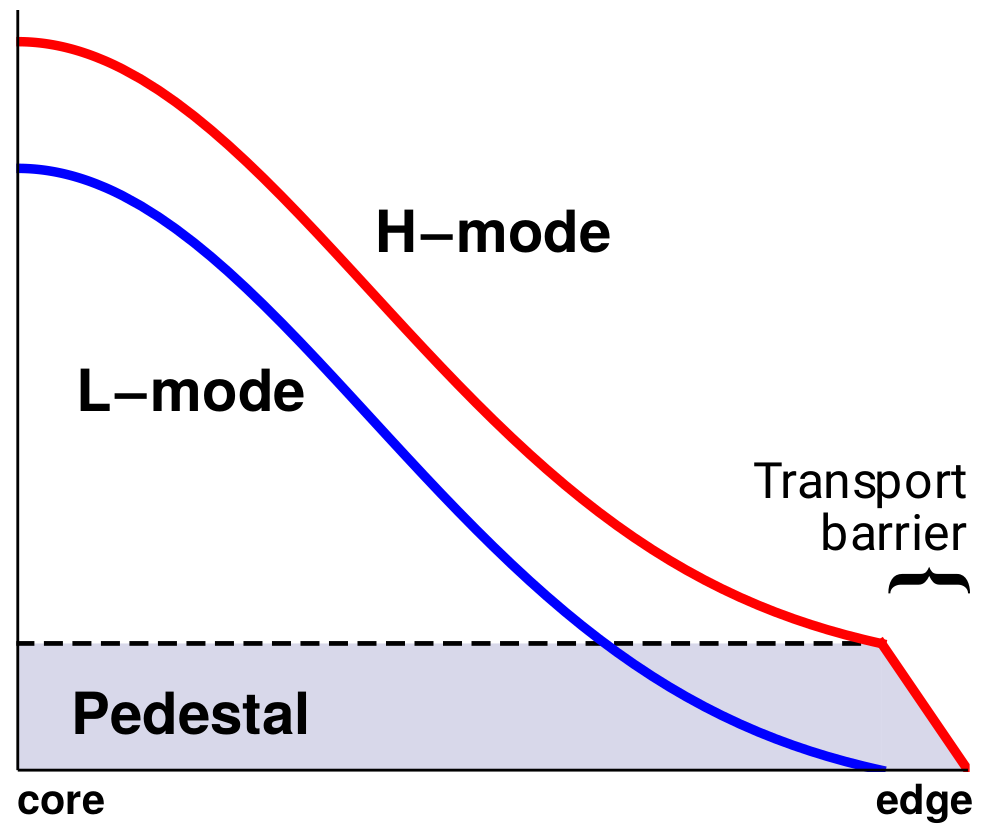
\includegraphics[width=0.8\textwidth]{../Graphics/L-mode_H-mode_compare.png}
\end{minipage}
\hfill
\begin{minipage}{0.49\linewidth}
	\caption{A comparison of the radial pressure profiles of L--mode and H--mode.
	The profile of H--mode can be thought of as on a `pedestal,' in which the pressure profile is increase in the core.
	This is due to the transport barrier that is formed at the edge \cite{weymiens_bifurcation_2014}.}
	\label{fig:L-mode_H-mode_compare}
\end{minipage}
\end{figure}

H--mode is characterized by its pressure profile significantly raised compared to that of L--mode, and is said to sit on a `pedestal.'
Accordingly, there is a steep gradient in the pressure at the edge of the plasma, shown and compared to L--mode in Figure~\ref{fig:L-mode_H-mode_compare} \cite{weymiens_bifurcation_2014}.
This results in an increased temperature in the core.

\section{The L--H Transition}
The key feature that determines a divertor tokamak's operational mode is the amount of external heating power.
Limiter tokamaks are relegated to stay in L--mode, as H--mode is an exclusive operating mode of tokamaks with divertors.
The transition has been observed to occur in one of three manners: sharp, smooth, and oscillatory.

\subsection{Bifurcation Theory}
A defining feature of L--H transitions is that they can occur very suddenly (the so-called sharp transition), which is characteristic of fold bifurcation behavior.
Mathematically, a bifurcation is defined to be a topological or qualitative change in a system when a small and smooth change of a parameter is made.
A simple example for a fold bifurcation is the following, with $a$ representing the parameter:
\begin{equation}
	\frac{\text{d}x}{\text{d}t} \,=\, \dot{x} \,=\, a + x^2.
	\label{eq:simple_fold}
\end{equation}
This equation can behave in one of three manners:
If $a > 0$, there are no real points of equilibrium, also known as steady-state solutions.
For $a = 0$, there is one equilibrium point at $x = 0$, and two for $a < 0$, with $x = \pm\sqrt{-a}$.
Varying $a$ from some positive real number to some negative number, the fundamental behavior of the solutions changes drastically at $a = 0$.
Equation~\ref{eq:simple_fold} is in the simplest known form of a fold bifurcation; the simplest form for any dynamical system is known as the topological norm form.
A phase plot of $x$ versus $a$ in Fig.~\ref{fig:simple_fold} illustrates this.

%{{{ Two figures for simple bifurcations (co-dimension 1)
\TwoFig{../Graphics/Bif_Graphs/Simple_fold.png}
	{Plot of parameter space for $\dot{x} = a + x^2$ (Eq.~\ref{eq:simple_fold}), with the co-dimension 1 bifurcation occurring at $a = 0$. %
	For $a < 0$, the system is unstable, and stable for points $a \geq 0$, shown in red and green, respectively.}
	{fig:simple_fold}
	{../Graphics/Bif_Graphs/co-2_fold.png}
	{Plot of parameter space for $\dot{x} = -(a + x - x^3)$ (Eq.~\ref{eq:sharp_bif}). %
	This system showcases two fold (co-dimension 1) bifurcations, at the turning points $a_{\pm\text{crit}}$, with two stable regions, in green and blue. %
	The red region is an intermediate that is unstable.}
	{fig:co-2_fold}
%}}}

%{{{ Two figures for zeros of the co-dimension 1 bifurcations
\TwoFigOneCap{../Graphics/Bif_Graphs/stationary_b-0_8.png}
	{../Graphics/Bif_Graphs/stationary_b_1_1.png}
	{Phase plots for Eq.~\ref{eq:sharp_bif}, with different values of $a$ within each plot. %
	There is a variance in the number of zeros based on the values of $a$ in the right plot, while there is strictly one zero for all values of $a$ in the left plot. %
	When there is multiple roots, the middle zero is always unstable.}
	{fig:stationaries_b}
%}}}

The co-dimension of a system refers to the lowest number of parameters required to produce the topological norm form.
Put differently, it is the number of parameters that must be varied for the bifurcation to occur.
In the case of Eq.~\ref{eq:simple_fold}, the co-dimension is one, and is thus referred to as a co-dimension 1 bifurcation \cite{weymiens_bifurcation_2014}.

\todo{\color{red}{FIX HERE!}}
The dynamic behavior of the L--H transition correspond very closely to a few certain bifurcations.
Work by Weymiens proves that the ``co-dimension 3 bifurcation robustly connects the three types of transition behaviour" and investigates using the FitzHugh-Nagumo model \cite{weymiens_bifurcation_2014}.

Physically, the transition is a bifurcation in the turbulent transport at the edge of the tokamak.
Sharp and smooth transitions are features of the cusp bifurcation, a two-fold bifurcation \cite{weymiens_bifurcation_2014}. 
The topological norm form of this behavior is
\begin{equation}
	\dot{x} \,=\, -(a + bx - x^3)
	\label{eq:sharp_bif}
\end{equation}

These two dynamics are distinguished only by density as the parameter.
The most common transition is the sharp transition, as the plasma parameters for it are more ideal for achieving fusion.

%{{{ Two figures for complex bifurcations
\TwoFig{../Graphics/Bif_Graphs/Bif_3D.png}
	{Two codimension 1 fold bifurcations, with the parameter $b$ dictating the size of the hysteresis, until the bifurcations merge into a cusp \cite{weymiens_bifurcation_2014}.}
	{fig:Bif_3D}
	{../Graphics/Bif_Graphs/3_transitions_single_simple.png}
	{Codimension 3 parameter space with the black line indicating the fold bifurcation. The parameter $b$ dictates the type of transition, including the size of the hysteresis in the sharp transition \cite{weymiens_bifurcation_2014}.}
	{fig:Bif_types}
%}}}

The third type of transition dynamics is oscillatory, also known as dithering.
These oscillatory solutions will only occur in the region near the cusp bifurcation point.

All three bifurcations are shown in parameter space in Fig.~\ref{fig:Bif_types}, with $b$ dictating the type \cite{weymiens_bifurcation_2014}.

\subsection{Hysteresis}
Hysteresis is a characteristic of any system which the current state of the system depends on its history.
The threshold power for the H--L transition is significantly lower than that of the L--H transition, leading to a region in which there is a non-unique solution to the plasma state.
This requires two separate fold bifurcations each to govern the L--H and H--L transitions separately, which in turn, requires two types of bifurcation parameters.
The first dictates hysteresis is present at all in the system; varying this allows for the disappearance of hysteresis when the aforementioned two fold bifurcations merge into a cusp bifurcation.
Varying the second parameter can cause the two stable solutions to be replaced by with unstable solutions, in which the system will oscillate between the solutions.
This phenomenon is called limit cycle oscillations; it is a result of a Hopf bifurcation \cite{weymiens_bifurcation_2014}.

\section{Mechanisms}
The prevailing hypothesis for the overarching mechanism for H--mode is that high auxiliary power develops strong sheared plasma flow and suppresses transport \cite{freidberg_plasma_2007}.

The shear stress dissociates smaller turbulent structures, with their energy and momenta transferred to larger flows \cite{staps_backstepping_2017}.
An accepted key mechanism for the transition is the generation of a large radial electric field and the corresponding $\mathbf{E}\times\mathbf{B}$ flows near the edge.
A plethora of individual processes for the generation of such an electric field have been proposed, most of which can be viewed as separate contributions in a radial Poisson's law, with some that tend to reduce the field.

The radial electric field $E_r$ is deduced from the radial force balance for any plasma species $j$, as follows:
\begin{equation}
	E_r \,=\, -\frac{1}{n_j e_j} \frac{\text{d} p_j}{\text{d} r} + V_{\theta j} B_\phi - V_{\phi j} B_\theta
	\label{eq:E_r}
\end{equation}
In the above, $e_j$ represents the charge of the $j$-th species, $n_j$ is the density, $p_j$ is the pressure, and $V_{\theta j}$ and $V_{\phi j}$ are the poloidal and toroidal velocities, respectively.
This grants changes in the radial electric field to be associated with changes in radial gradient of the pressure or either velocities \cite{connor_review_2000}\cite{staps_backstepping_2017}.
However, determining these values is difficult due to large possible error in experiment.

\section{Research Questions}
Although there have been compilations of different theories describing the transition, there is yet to be a conclusive, comprehensive one \cite{connor_review_2000}.
There is substantial evidence, both theoretically and experimentally, that a radial electric field is an integral piece in the forming and enforcing of H--mode.
Many of the effects in generating and suppressing the field show up as additive terms in an equation for a radial displacement current.
Because many of these fluxes scale differently, simple scaling laws for H--mode could contrast for regimes where different effects dominate.
It is therefore important to evaluate which terms dominate in their respective regimes before inquiring about global scalings.
The overall problem is thus stated simply: \textbf{Which electric field-generating terms are dominant in concrete experimental tokamak conditions?}
This is in an effort to determine which measurable and controllable values can predict H--mode.

The first consideration is to decide \textbf{which terms should be considered for investigation}, as not all nonambipolar fluxes will significantly contribute to the transition.
For example, the nonambipolar flux due to magnetic ripple loss highly depends on collisionality, in which lower collisionality results in a low flux \cite{stringer_ripple_1972}.
Since a relatively ideal operation (temperature on the order of 1 keV at the edge) will be investigated, this flux can be neglected.

\textbf{Identifying what optimal form and relative strengths of each flux and subsequently implementing them} appropriately is the crucial next step.
Because the model is highly nonlinear, it is sensitive to the forms and relative strengths.
The calculation is done with a finite volume method solver, in which the results requires verification with the literature.

The main input heating power regime previously investigate was strictly limited to near the H--L transition \cite{staps_backstepping_2017}.
Performing a scan of input heating power significantly above the lower threshold could show a difference in behavior of the fluxes and resulting field.
Therefore, \textbf{what is the variation in dominance of each field-generating term across increasing input power}, including those inside and outside the regime with non-unique operational modes?

